\documentclass[pdf,xcolor=dvipsnames,noparindent]{beamer}

\usetheme{Warsaw}
\usecolortheme{spruce}

% packages
\usepackage{listings}
% \usepackage{upquote}

% \lstset{numbers=left, numberstyle=\footnotesize, stepnumber=1,firstnumber=1,
%     numbersep=5pt,
%     stringstyle=5pt,
%     basicstyle=\footnotesize,
%     keepspaces=true, tabsize=4,
%     showstringspaces=false
%     % backgroundcolor=\color{SpringGreen}
% }

% preamble
\title{Introduction to Go - Part 1}
\author{Wojciech Gac}
\date{July 26, 2019}

% document proper
\begin{document}

\begin{frame}
	\titlepage
\end{frame}

% \begin{frame}{Outline}
% 	\pause
% 	\begin{itemize}
% 		\item The Problem
% 		      \pause
% 		\item Delve Debugger
% 		      \pause
% 		\item Container Preparation
% 		      \pause
% 		\item Debugging
% 		      \pause
% 		\item Further Reading
% 	\end{itemize}
% \end{frame}

% \begin{frame}
% 	\frametitle{The Problem}
% 	We'd like to be able to do the following:
% 	\pause
% 	\begin{itemize}
% 		\item Using a local instance of VSCode...
% 		      \pause
% 		\item ...and a dockerized instance of a Go application...
% 		      \pause
% 		\item ...connect to a running process \emph{inside} the container...
% 		      \pause
% 		\item ...interrupt execution with breakpoints and modify variables on the fly
% 	\end{itemize}
	  
% \end{frame}

\begin{frame}{Outline}
  \pause
  \begin{itemize}
  \item Origins of Go
    \pause
  \item Language Basics
    \pause
  \item Patterns
    \pause
  % \item Concurrency Patterns
    % \pause
  \item Practical Use Cases
    \pause
  \end{itemize}
\end{frame}

\begin{frame}{Origins of Go}
  \pause
  \begin{itemize}
  \item Designed at Google in 2007
    \pause
  \item ... by Rob Pike, Ken Thompson and Robert Griesemer
    \pause
  \item ... two of whom (Pike \& Thompson) had spent decates at Bell Labs
    \pause
  \item ... building on a long history of concurrent languages
    \pause
  \item ... such as Occam, Erlang, Newsqueak, Concurrent ML, Alef and Limbo
  \end{itemize}
  
\end{frame}

\begin{frame}{Origins of Go}
  \pause
  \begin{itemize}
  \item Heavily influenced by Tony Hoare's CSP paper from 1978
    \begin{figure}
      \centering
      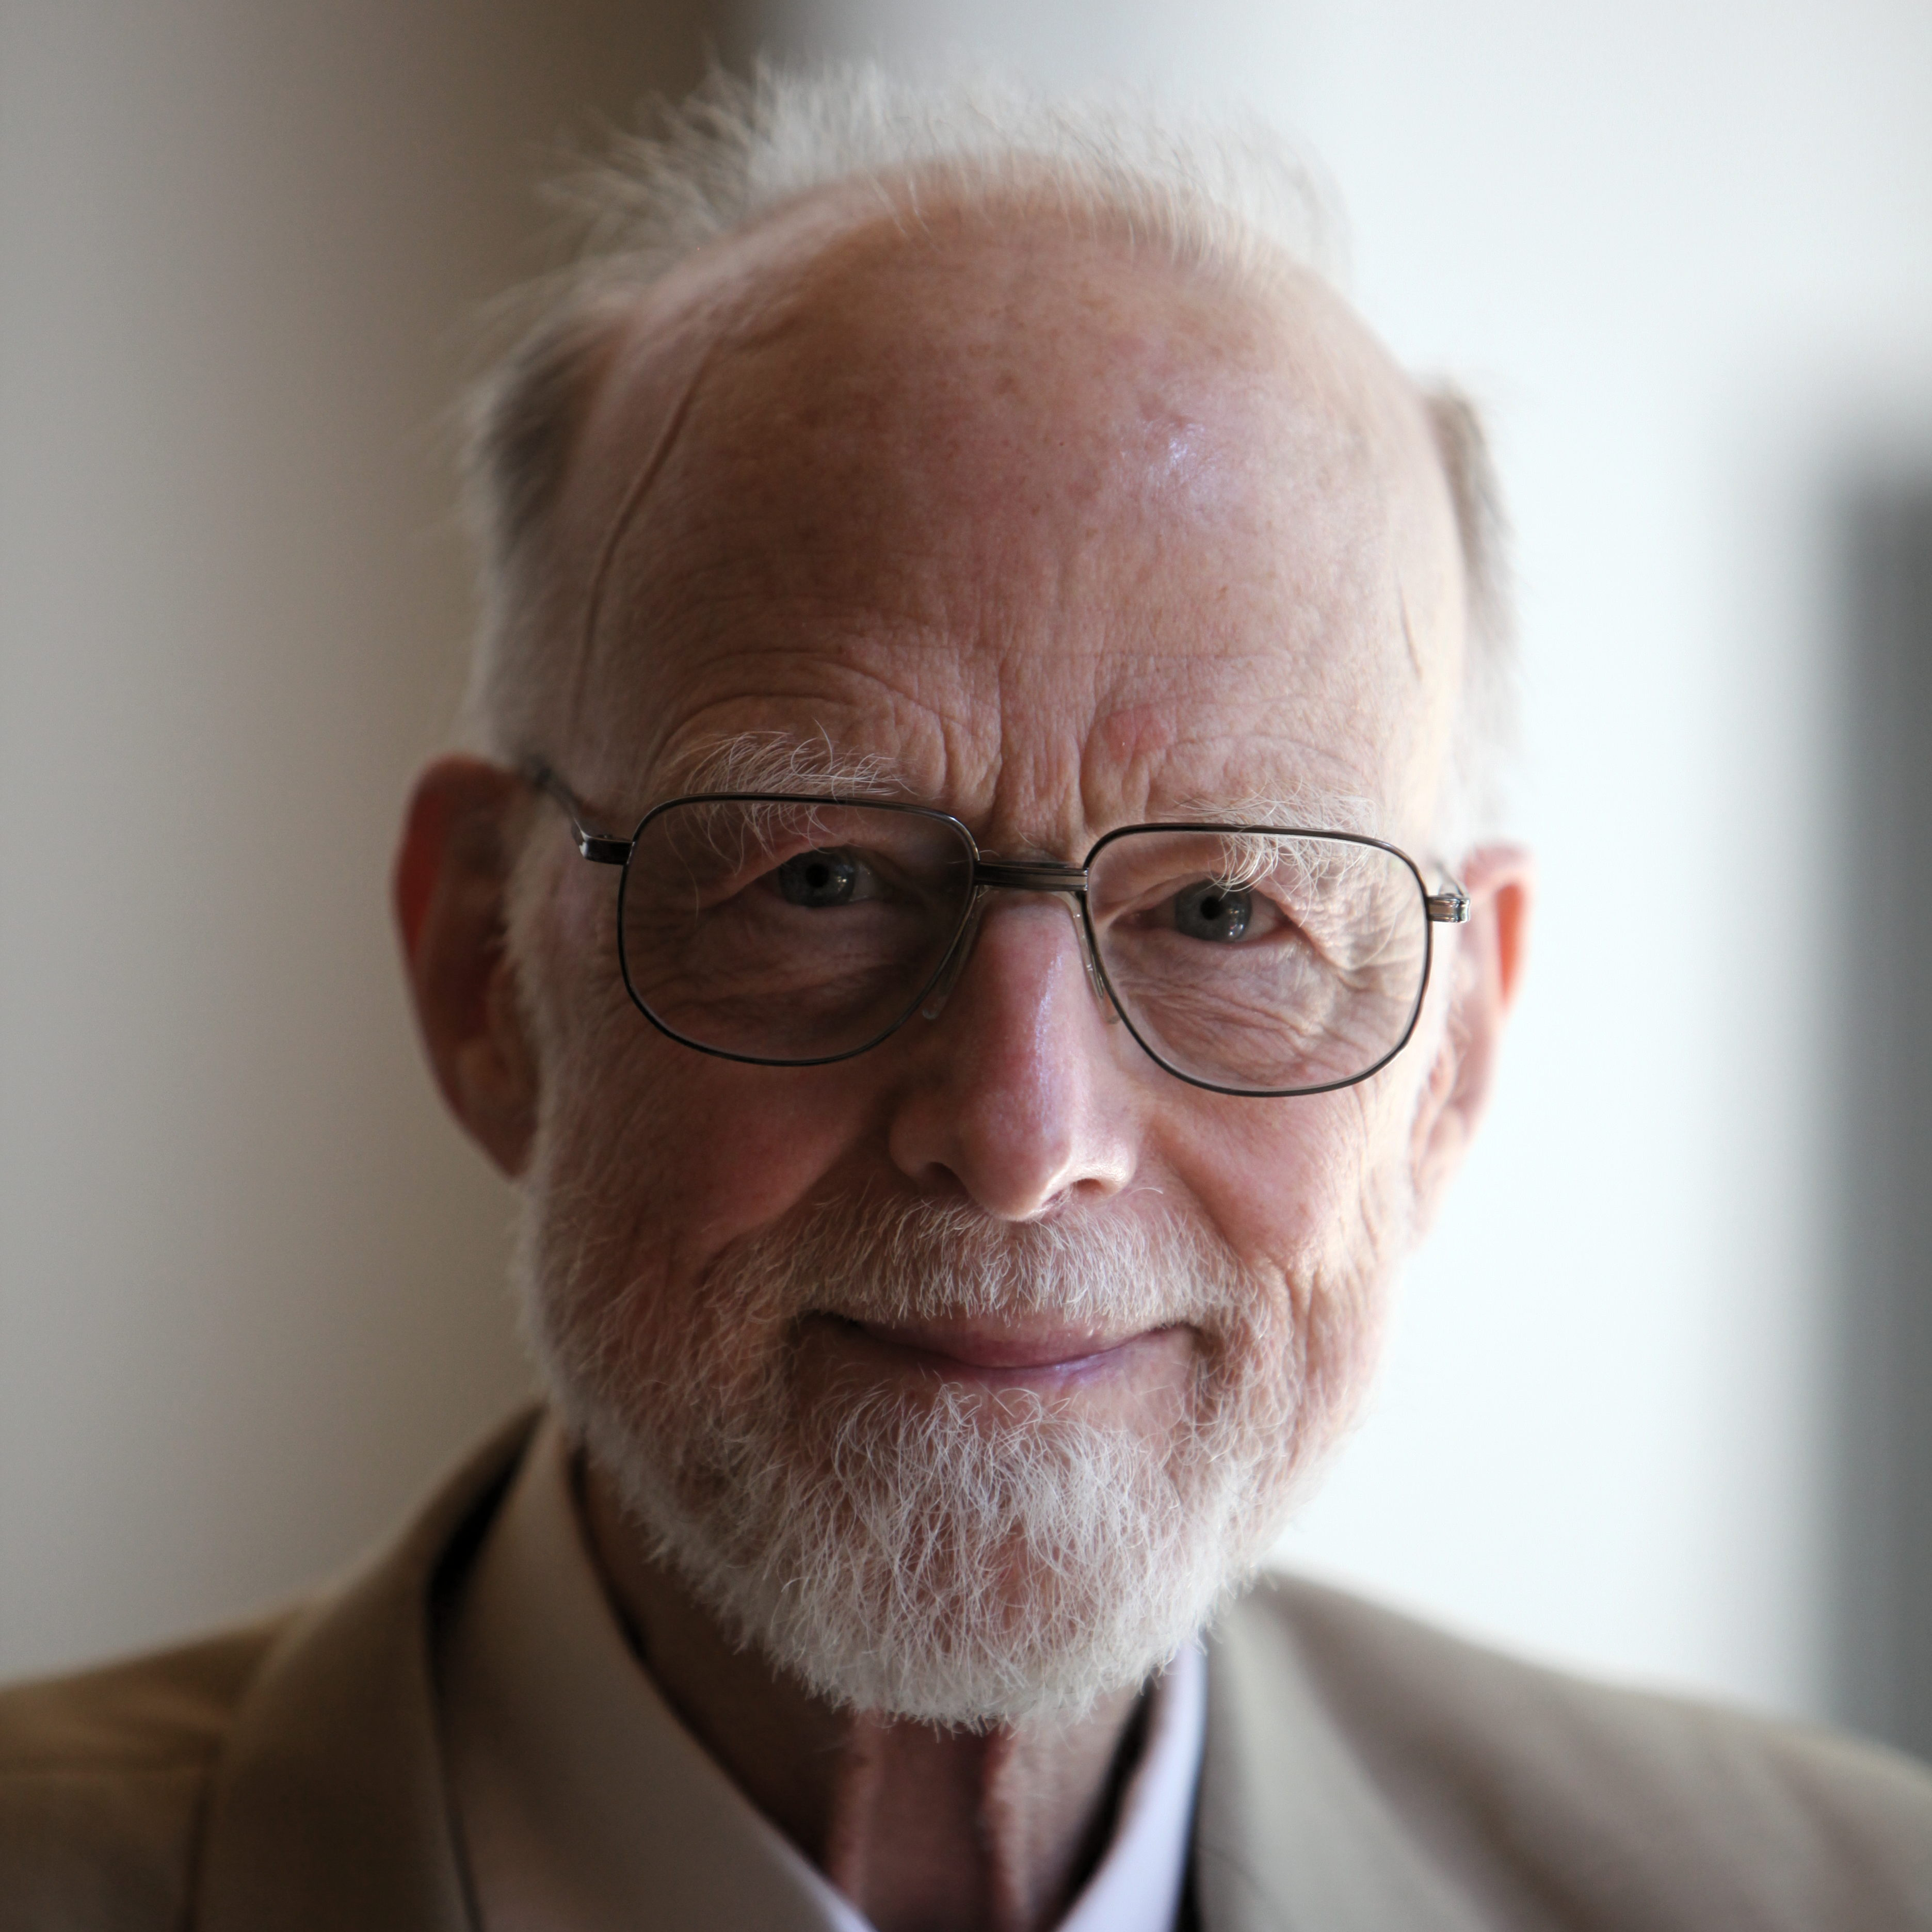
\includegraphics[scale = 0.02]{images/hoare.jpg}
    \end{figure}
    \pause
  \item ... in which input and output operations are programming primitives
    \pause
  \item ... helping structure parallel process communication
  \end{itemize}
  
\end{frame}

\begin{frame}{Origins of Go}
  \pause
  Rationale:
  \pause
  \begin{itemize}
  \item C++ compile cycles took too long at Google
    \pause
  \item The C model was efficient, but lacked more modern facilities \& libraries
    \pause
  \item A fast, compiled, no-nonsense systems programming language was needed
    \pause
  \item Memory safety, garbage collection, structural typing and concurrency were prioritized
    \pause
  \item Module/namespace system facilitated development of very large systems without name collisions
    \pause
  \item Good style had to be formalized to avoid ambiguity
  \end{itemize}
\end{frame}

\begin{frame}{Origins of Go}
  \pause
  Things happen fast...\\
  \pause
  ...when you're backed by Google
\end{frame}

\begin{frame}{Origins of Go}
  \pause
  A (very) incomplete list of adopters:
  \begin{itemize}
  \item Docker
    \pause
  \item Dropbox
    \pause
  \item Uber
    \pause
  \item Cloud Foundry
    \pause
  \item Ethereum
    \pause
  \item Netflix
    \pause
  \item Heroku
    \pause
  \item MongoDB
    \pause
  \item Allegro
    \pause
  \item OLX
    \pause
  \item Yandex.ru
    \pause
  \item Google - obviously
  \end{itemize}
\end{frame}

\begin{frame}{Language Basics}
  \pause
  Language attributes:
  \begin{itemize}
    \pause
  \item Compiled to native code
    \pause
  \item Garbage collection
    \pause
  \item Statically typed
    \pause
  \item Syntax similar to C
    \pause
  \item Rich default toolchain
    \pause
  \item Official formatting style (enforced by the compiler)
    \pause
  \item Simplified model of OOP (structs, methods, interfaces)
  \end{itemize}
\end{frame}

\begin{frame}{Language Basics}
  Integrated tooling:
  \pause
  \begin{itemize}
  \item \texttt{go build} - build tool
    \pause
  \item \texttt{go test} - run tests
    \pause
  \item \texttt{go fmt} - format source code
    \pause
  \item \texttt{go get} - retrieve external packages
    \pause
  \item \texttt{go vet} - static code analyzer
    \pause
  \item \texttt{go run} - run code
    \pause
  \item \texttt{godoc} - documentation tool
    \pause
  \item \texttt{gorename} - safe renaming tool
  \end{itemize}
\end{frame}

\begin{frame}[fragile]{Language Basics}
  \pause
  Variables:
  \pause
  \begin{itemize}
  \item Variable declaration:
    \begin{semiverbatim}
      var <name> <type>
    \end{semiverbatim}
    \pause
  \item Variable assignment:
    \begin{semiverbatim}
      <name> = <value>
    \end{semiverbatim}
    \pause
  \item Combined declaration \& assignment:
    \begin{semiverbatim}
      var <name> <type> = <value>
    \end{semiverbatim}
    \pause
  \item Short declaration with type inference (a'la C++ \texttt{auto}):
    \begin{semiverbatim}
      <name> := <value>
    \end{semiverbatim}
  \end{itemize}
\end{frame}

\begin{frame}{Language Basics}
  \pause
  Basic data types:
  \pause
  \begin{itemize}
    \begin{columns}
      \column{0.4\textwidth}
    \item \texttt{int}
    \item \texttt{int8}
    \item \texttt{int16}
    \item \texttt{int32}
    \item \texttt{int64}
      \pause
    \item \texttt{uint}
    \item \texttt{uint8}
    \item \texttt{uint16}
    \item \texttt{uint32}
    \item \texttt{uint64}
    \item \texttt{uintptr}
      \pause
      \column{0.4\textwidth}
    \item \texttt{bool}
      \pause
    \item \texttt{string}
      \pause
    \item \texttt{byte}
    \item \texttt{rune}
      \pause
    \item \texttt{float32}
    \item \texttt{float64}
      \pause
    \item \texttt{complex64}
    \item \texttt{complex128}
      \end{columns}
  \end{itemize}
\end{frame}

\begin{frame}[fragile]{Language Basics}
  Function definitions:
  \pause
  \begin{verbatim}
func <name>(<parameters>...) <return-types>... {
  // body... 
  
  // optional
  return <return-value>
}
\end{verbatim}
  \pause
  Anonymous functions are identical, except for \texttt{<name>}
\end{frame}

\begin{frame}[fragile]{Language Basics}
  Arrays:
  \pause
\begin{verbatim}
// Array declaration
var arr [10]int64

// Array quick declaration, initialized
arr := [5]int64{1, 2, 3, 10, 20}

// Array quick declaration, length inference
arr := [...]int64{1, 2, 3, 10, 20}
\end{verbatim}
\end{frame}

\begin{frame}[fragile]{Language Basics}
  Slices (like arrays, only better):
  \pause
\begin{verbatim}
// Slice declaration
arr := make([]int64, 10)

// Slice quick declaration, initialized
arr := []int64{1, 2, 3, 10, 20}

// Extend slice by appending
arr = append(arr, 10)

// Append another slice
arr = append(arr, arr2...)
\end{verbatim}
\end{frame}

\begin{frame}[fragile]{Language Basics}
  Structures:
  \pause
\begin{verbatim}
type person struct {
  firstName string
  lastName  string
  sex       string
}

jasiu := person{
  firstName: "Jan",
  lastName:  "Kowalski",
  sex:       "Yes, please",
}

fmt.Printf("Name: %s %s Sex: %s\n",
  jasiu.firstName, jasiu.lastName, jasiu.sex,
)
\end{verbatim}
\end{frame}

\begin{frame}[fragile]{Language Basics}
  Maps:
  \pause
\begin{verbatim}
// Empty map
m := make(map[string]int)

// Key lookup
val, ok := m["key"]

// Delete key
delete(m, "key")

// Map literal
m := map[string]int{"a": 1, "b": 2, "c": 3}
\end{verbatim}
\end{frame}

\begin{frame}[fragile]{Language Basics}
  Channels:
  \pause
  \begin{itemize}
  \item Implementation of Hoare's CSP
    \pause
  \item Two way, typed pipes (unbuffered by default)
    \pause
  \item Blocking write until there is a reader
    \pause
  \item ...and read until there is a writer
    \pause
  \item Fundamental building blocks of concurrency in Go
  \end{itemize}
  
\end{frame}

\begin{frame}[fragile]{Language Basics}
  Channels (continued):
  \pause
\begin{verbatim}
// Create channel
ch := make(chan int64)

// Write to channel (blocking)
ch <- 12343

// Read from channel (blocking)
<-ch
\end{verbatim}
\end{frame}

\begin{frame}[fragile]{Language Basics}
  Goroutines:
  \pause
  \begin{itemize}
  \item Background functions, multiplexed onto (but not identical with) threads
    \pause
  \item Can be thought of as lightweight threads
    \pause
  \item Decoupled from the main program unless channels are used
    \pause
  \item Can be instantiated by the thousands (millions maybe?)
  \end{itemize}
\end{frame}

% \begin{frame}[fragile]{Language Basics}
%   Testing:
%   \pause
%   \begin{itemize}
%   \item Tests for \texttt{file} are in \texttt{file_test}
%     \pause
%   \item Tests are defined as follows:
% \begin{verbatim}
% func Test...(t *testing.T) {
%   ...
% }
% \end{verbatim}
%   \end{itemize}
% \end{frame}

\begin{frame}[fragile]{Patterns}
  Multiple return values:
  \pause
\begin{verbatim}
func divAndMod(a, b int) (int, int) {
  return a/b, a%b
}
...
div, mod := divAndMod(10, 3)
fmt.Printf("Quotient: \%d Remainder: \%d\n", div, mod)
\end{verbatim}
  
\end{frame}

\begin{frame}[fragile]{Patterns}
  Error handling:
  \pause
\begin{verbatim}
func div(a, b int) (int, error) {
  if b == 0 {
    return 0, errors.New("Division by zero")
  }
  return a / b, nil
}
...
q, err := div(10, 20)
if err != nil {
  fmt.Errorf("Error performing division: %v", err)
}
\end{verbatim}
\end{frame}

\begin{frame}[fragile]{Patterns}
  Fan-in with channels:
  \pause
\begin{verbatim}
func fanIn(input1, input2 <-chan string) <-chan string {
    c := make(chan string)
    go func() {
        for {
            select {
            case s := <-input1:  c <- s
            case s := <-input2:  c <- s
            }
        }
    }()
    return c
}
\end{verbatim}
\end{frame}

\end{document}